The Discontinuous Galerkin method results in truncation error that scales as $h^{N+1}$, where $h$ is the element size and $N$ is the order of the interpolating polynomials within the element.~\cite{dghesthaven} The self force is given by the radial derivative of the 


Note that it is not always possible to choose three points such that they lie on a converging exponential form, for instance, if they are not monotonic, or if they curve in the wrong direction. In these cases, I say that the ``mode failed'', and discard the result for that mode with that starting order for the extrapolation. I use extrapolation starting orders from the set 12, 16, 20, 24, 28, 32, and 36, with additional data at orders 40 and 44 that may be used as points two and three in the extrapolation. 

\begin{figure}
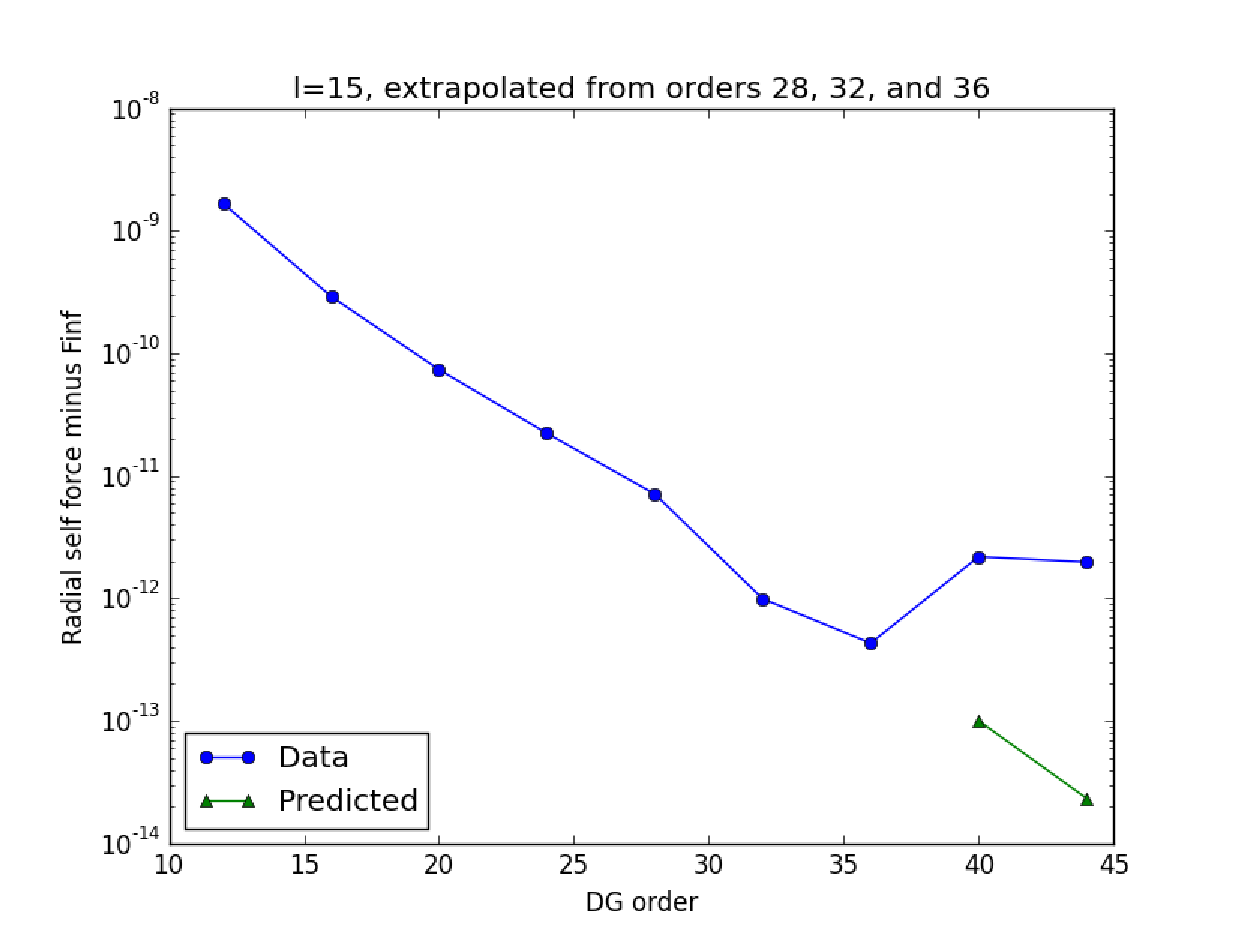
\includegraphics{extrapolate7plot}
\caption{DG convergence with order, extrapolated from highlighted points to infinite order along exponential form, which appears as a straight line in the semilog plot.}
\end{figure}



\begin{figure}
  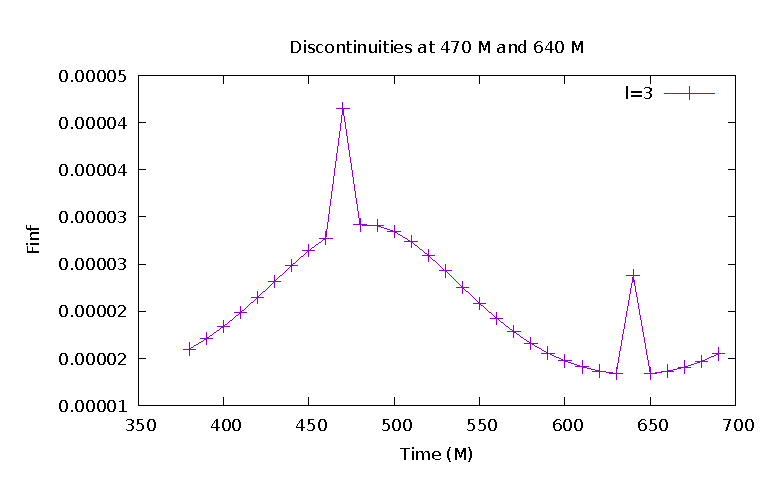
\includegraphics{finfovertimel3discontinuities}
  \caption{Starting order was chosen by iterating from the lowest order to the first order for which the ``mode failed'', and chosing the maximum starting order that succeded. When $F_{\inf}$ is evolved over one full orbital cycle, some l-modes shows discontinuities at some times. l=3}
\end{figure}




\begin{table}
  \begin{tabular}{lll}
    time & starting order & finf\\
    632 & 0 & mode failed\\
    632 & 1 & 2.40975299617e-05\\
    632 & 2 & 2.40975300465e-05\\
    632 & 3 & 2.40975300114e-05\\
    632 & 4 & mode failed\\
    632 & 5 & 2.40975299291e-05\\
    632 & 6 & 2.40975299148e-05\\
  \end{tabular}
  \caption{Manual starting indices and $F_{\inf}$ values for t=632, l=2.}
  \label{manual}
\end{table}

\begin{figure}
  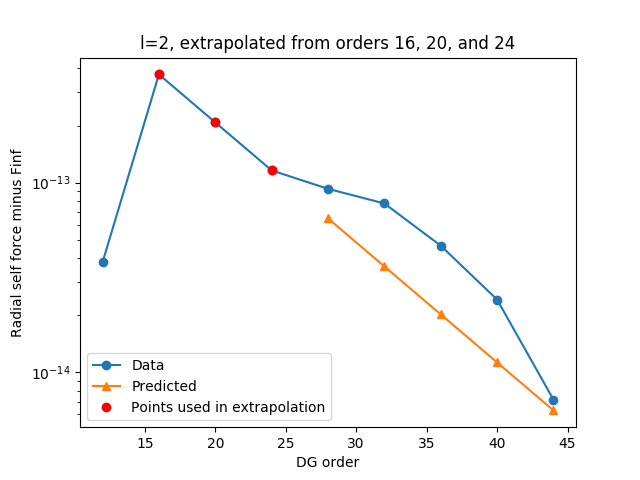
\includegraphics{extrapolate7t632l2i1}
  \caption{Fluctuation in one of the points chosen in the extrapolation, due to roundoff or truncation error, causes the extrapolation to predict a value of $F_{\inf}$ that is subtly wrong, leading to curvature in the semilog plot after $F_{\inf}$ subtraction. t=632, l=2, i=1}
\end{figure}

\begin{figure}
  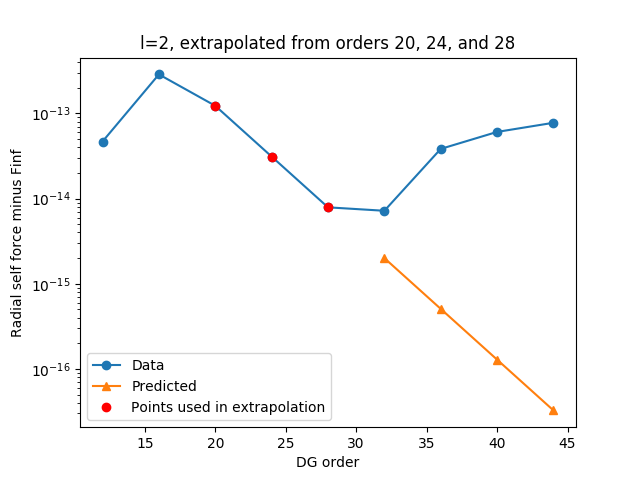
\includegraphics{extrapolate7t632l2i2}
  \caption{Roundoff error is visible at high DG orders. t=632, l=2, i=2}
\end{figure}

\begin{figure}
  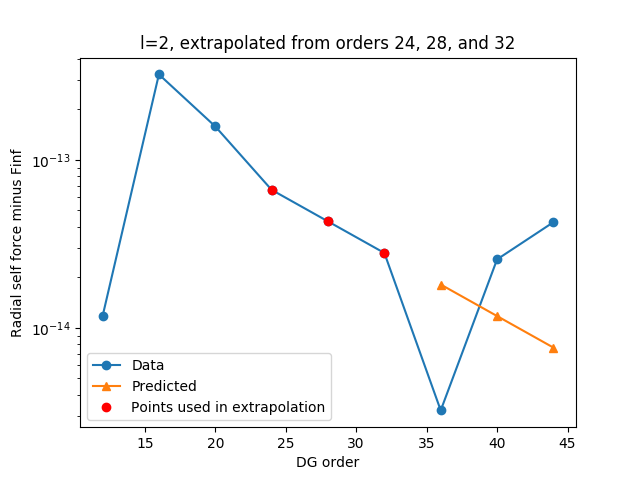
\includegraphics{extrapolate7t632l2i3}
  \caption{The incorrect value of $F_{\inf}$ has been chosen due to roundoff error, perhaps due to finite precision in the root finding algorithm, leading to a negative values, that show as a ``V'' in the semilog plot. t=632, l=3, i=3}
\end{figure}


\begin{figure}
  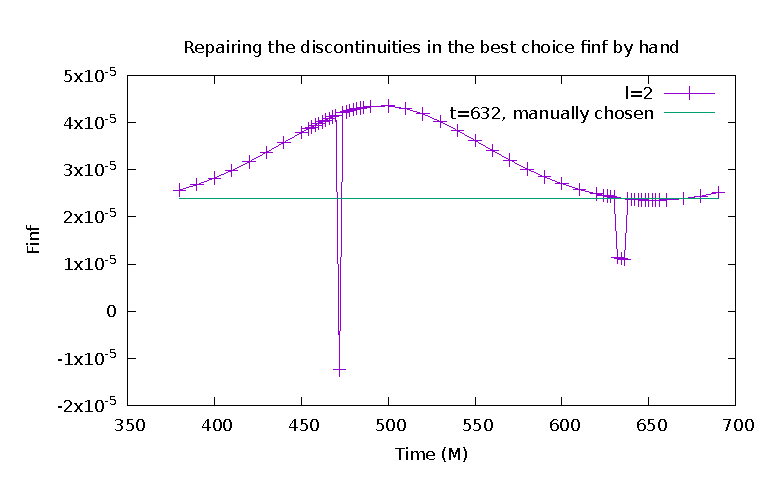
\includegraphics{bestFinfManuallyChosent632l2}
\caption{Manual correction for the discontinuities in the l=2 mode, using the manually determined $F_{\inf}$ data from Table~\ref{manual}. }
\end{figure}

\subsection{ Checking for discontinuities in $F_{\inf}$ for each each l-mode}

In the median approach, the starting orders that did not ``fail'' at each time and for each mode are ordered by their $F_{\inf}$ values. The median value of $F_{\inf}$ is selected, presumably discarding those effected by roundoff and those effected by failure to converge. However, there is no guarantee that it selects those in this regime, since in principle a mode could both be in the roundoff limit and have not converged yet. Yet when this is done, there are no discontinuities in $F_{\inf}$ for any of the l-modes when the median approach is used. See mode zero for an example.

\begin{figure}
  \includegraphics{finfovertimel0}
  \caption{An example of no discontinuities in $F_{\inf}$ for any of the l-modes. Mode $l=0$.}
\end{figure}


\subsection{Determining $F_{\inf}$ using maximum likelihood fits to subsegments of lines in semilog space}
A better motivated approach, is to fit subsegments of lines in semilog space onthe DG order convergence plot, and find the most linear, longest linear, region. A fit with the ``best'' value of the reduced chi squared should be a good approximation to this. The reduced chi squared is the value of the sum of the residuals of the fit squared divided by the number of degrees of freedom, which in this case is the number of points in the fit minus two, since there are two degrees of freedom in a linear fit. The expectation value of the reduced chi squared, in the limit of a large number of degrees of freedom, is one. I loop over starting and ending points of the fit, and over starting orders, and choose the starting order with the best fit line segment in the sense that that line segment has a reduced chi squared closest to one. An example of such an automatically chosen starting index is given in Figure~\ref{autoconverge}, where there is a long exponentially converging region.

\begin{figure}
  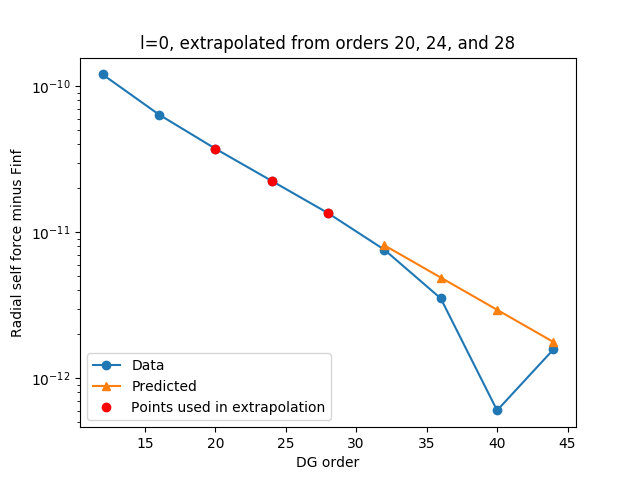
\includegraphics{fittingtechniqet370l0}
  \caption{l=0 mode with line-segment fit-chosen starting order produces convergence plot with long exponentially converging region}
\end{figure}





